\section{Implementation}\label{impl}
This section overviews the implementation of SCache -- a distributed in-memory storage system that caches shuffle data of DAG framework. Here we use Spark as example of DAG framwork to illustrate working process of shuffle optimization. We will first present system architecture in Subsection \ref{arch} while the following two subsections focuss on the two constraints on memory manangement.

\subsection{System Architecture}\label{arch}
SCache consists mainly two components: A distributed in-memory shuffle data storage system and the daemon inside Spark. As shown in Figure \ref{fig:arch}, for the in-memory storage system, SCache employs the legacy master-slaves architecture like GFS\cite{gfs}. The master node of SCache coordinates the shuffle blocks globally with application context from Spark. The coordination provides two guarantees: (a)store data in memory before tasks start and (b)schedule data on-off memory with all-or-nothing property and context-aware-priority constraints to benifit all jobs. 

When a Spark job starts, the DAG will be first generated by Spark DAGScheduler\cite{sparksource}. The process starts on the last result stage, and recursively find the dependent stages until the beginning of the DAG. While going forward to the beginning, the DAG computing pipeline will be cut off if a RDD in the stage has one or more shuffle dependencies. These shuffle dependencies among RDDs will then be submitted through RPC call to SCache master by a daemon process in Spark driver. For each shuffle dependency, the shuffle ID(an integer generated by Spark), the type of partitioner, the number of map tasks and the number of reduce tasks are included in the RPC call. The SCache master will store the metadata of one RPC call as a set of mutilpule shuffles scheduling unit. If there is a specialized partitioner, such as Range Partitioner or a customed paritioner, in the shuffle dependencies, the daemon will insert a sampling program in the host RDD that generates shuffle output using specialized partitioner. The sampling application will be scheduled ahead of that host RDD. We will illustrate the sampling procedure in the Section \ref{sampling}.

For the hash partitioner, when the map tasks in a stage finish computing on the work nodes, the  SCache Worker Daemon process will hijack the shuffle map output in the JVM of each executor of Spark (see Figure \ref{fig:arch}). Then the data will be transfered into the reserved memory of SCache Worker on each node through memory copy. In the same time, the Spark tasks will end after the memory copy without the disk shuffle output writing, which leads to a  reduction of the whole tasks completion time. When the shuffle map output block of a task is stored in the reserved memory, the SCache worker will then notify the master of the block belonging information with the reduce size distribution in this block (see Map Output in Figure \ref{fig:shuffle}). When the collected map output data reach the observed raito of map output, the SCache master will then run the scheduling algorithm \ref{mhminheap} (for multiple shuffle dependencies) and \ref{hminheap} (for single shuffle dependency) to get the reduce tasks -- nodes mapping. When the scheduling resulted is made, the master will then notify each worker to prepare the memory space for the shuffle data for reduce tasks. The pre-fetch of shuffle data as soon as each worker receives the scheduling results. More specifically, each worker will check the ID of reduce tasks that will be scheduled on itself in the future. When a map task finishs, each node will receive a broadcast message. It will then trigger the pre-fetch process to start fetching shuffle data from the memory of remote SCache worker that just finishs the map task. After all blocks of shuffle map output is transferred, the SCache worker will flush these blocks to disks for saving memory space and fault tolerence. 

Before the reduce stage starts, Spark DAG Scheduler will first generate a task set for this stage with different locality levels -- \textbf{\textit{PROCESS\_LOCAL, NODE\_LOCAL, NO\_PREF, RACK\_LOCAL, ANY}}. The locality levels are set by finding a cached location of a RDD. For the RDDs that have narrow dependency(oppsite ot shuffle dependency), the prefered location can also be the same as the depedent RDDs. For those RDDs that have shuffle dependecies, the locality will be set as \textbf{\textit{NO\_PREF}} by default. To enforce SCache pre-allocated the reduce tasks, we insert some lines of codes in Spark DAG Scheduler to consult SCache Master to get the preferred node for each tasks. By doing this, the tasks with shuffle dependencies can be set as \textbf{\textit{NODE\_LOCAL}}. Then the Task Scheduler will schedule tasks according to the task -- node mapping from SCache. 

When the scheduled reduce tasks start, the shuffle input data is requested. The SCache worker will then pass the requested data through memory copy from the reserved memory to Spark executor JVM memory. As soon as the memory copy finishes, the data in reserved memory will then be flushed to the disk.

\subsubsection{Reservior Sampling}\label{sampling}
If the submitted shuffle dependencies contain a Rrange Partitioner or a customed partitioner, the SCache master will send a sampling request to the daemon process in Spark driver. The daemon process will then submit a job on Spark for the current RDD. This sampling job will use a reservoir sampling algorithm\cite{reservoir} on each partition of RDD since the items size of each partition is unknow before sampling. For the sample number, we set the size equals to $3 \times number\ of\ partitions$ for balancing overhead and accurancy (it can be tuned by configuration). The sampling job will then perform a local shuffle with the selected items and partitioner (see Figure \ref{fig:sample}). At the same time, the size of items is counted as the weight of each partition.These sampling data will be aggregated by $reduce\ ID$on SCache master. The size for each reduce partition can be easily computed by equation \ref{equationsample}. After the prediction, master will call algorithm \ref{mhminheap} and \ref{hminheap} to do the scheduling. 

\begin{figure}
	\centering
	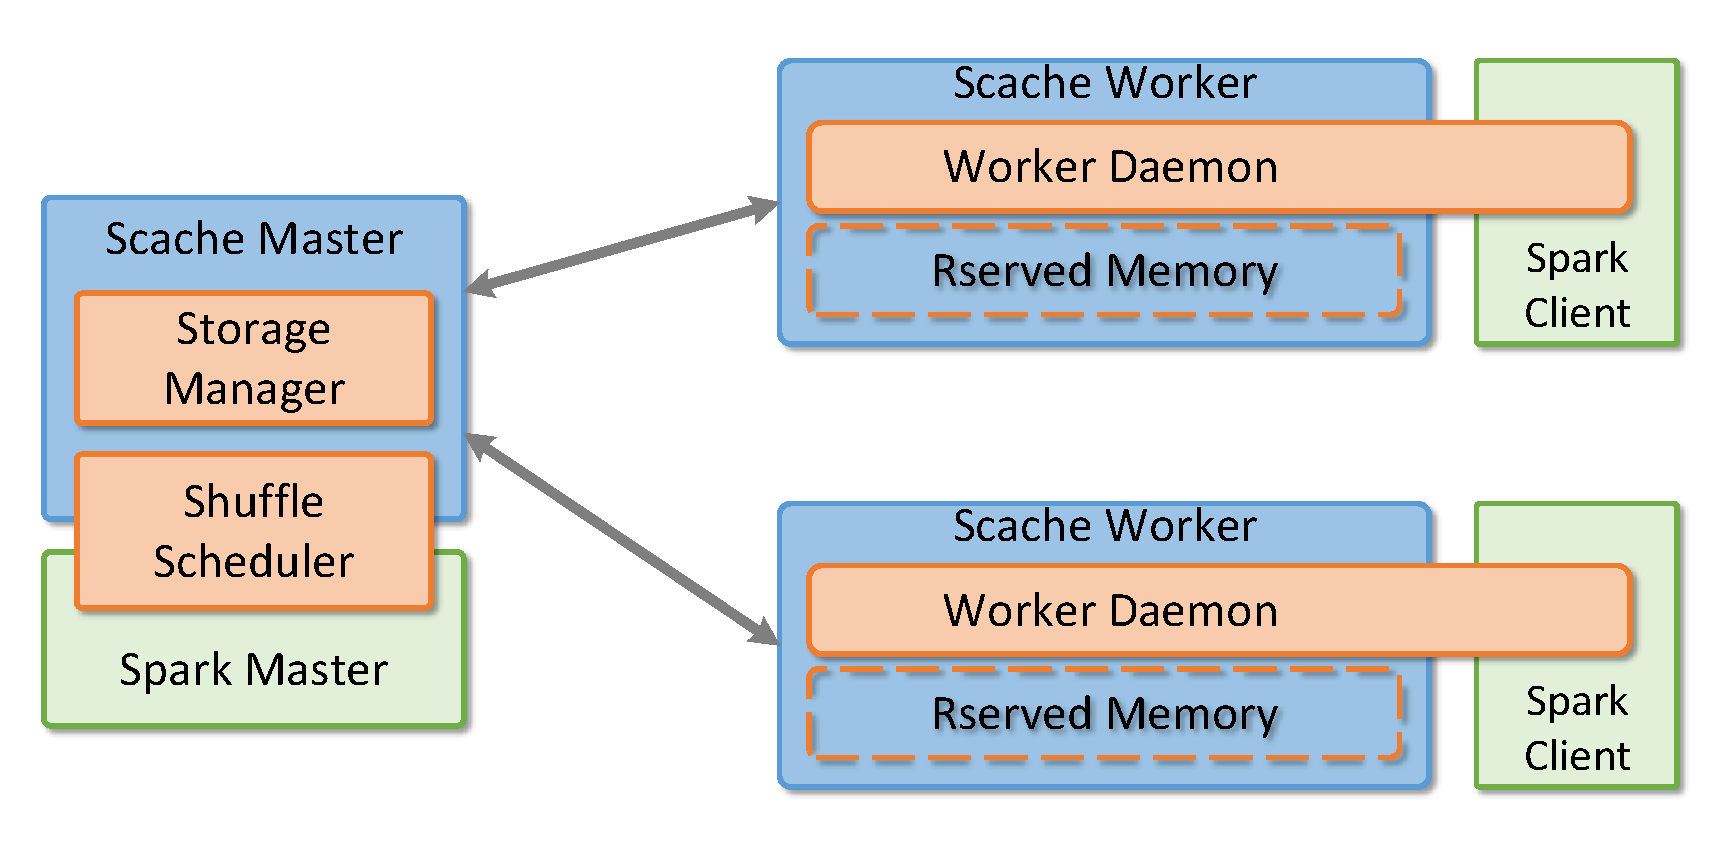
\includegraphics[width=\linewidth]{fig/arch}
	\caption{SCache Architecture}
	\label{fig:arch}
\end{figure}
\begin{figure}
	\centering
	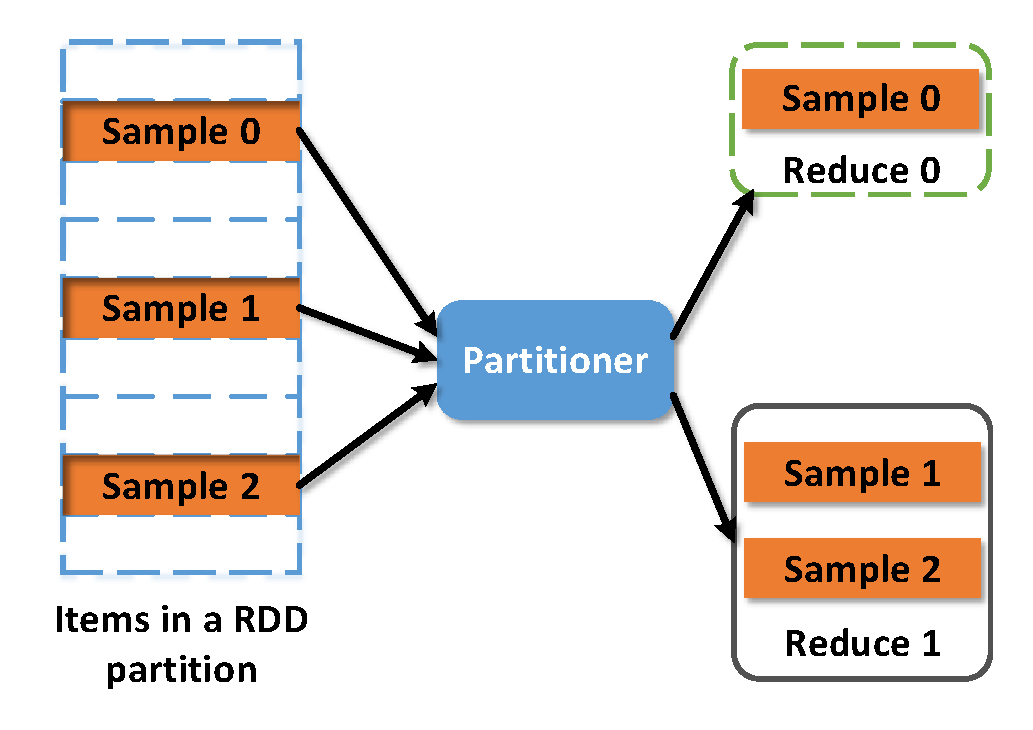
\includegraphics[width=\linewidth]{fig/sample}
	\caption{Reservoir Sampling of One Partition}
	\label{fig:sample}
\end{figure}

\subsection{Memory Management}
As mentioned in section \ref{shufflesize}, the shuffle size is small enough that can be easily fit in memory. In order to minimize the reserved memory of SCache worker on each node or configure the wrong size by user, the probablity of memory exceeded is still exist, especially for multipule existing applicaitons scenrios. When the cached data meet the limitaion of reserved memory, SCache flushes some of them to the disk temporarily. And refetch them as soon as some cached shuffle blocks is consumed by tasks. To achieve maximum imporvment in overall, SCache leverages two constraints to manage the in-memory data -- all-or-nothing and  context-aware-priority property.
\subsubsection{All-or-Nothing Property}
Achieving memory cached shuffle data for a reduce task will shorten the task execution time. But this acceleration of single task doesn't speed up the whole stage. Base on the observation that in most cases one single stage contains multi-rounds of tasks from section \ref{multi}, the shuffle cache should at least benifit all tasks in one round. If one of the task misses a memory cache and exceeds the original bottleneck of this round, that task will become the new bottleneck of that round and can further slow down the whole stage. PACMan\cite{pacman} has prooved that for multi-round stage/job, the completion times imporves in setps when $n\times number\ of\ tasks\ in\ one\ round$ tasks have data cached in local memory. Therefore, the memory cache of shuffle data need to match at least every round of tasks in a stage. We refer to this as the all-or-noting property. 

According to all-or-nothing property, SCache master leverages the scheduled results to determine the bound of each round of tasks, and then use this as the minimum unit of storage to manage the reserved memory globally. That is, there is one or more storage units for a shuffle schedule unit \textcolor{red}{add figure}. For those incomplete unit, SCache will mark them as the lowest priority. Following the all-or-noting contraint can maximum the improvement in stage completion time by using reserved memory efficiently.

\subsubsection{Context-Aware-Priority Property}
When the size of cached shuffle data exceeds the reserved memory, SCache should decide which of these should be flushed to disk according to the priorities of each storage unit. SCache master first searches if there is an incomplete unit and flush all blocks belonging to the unit to disk cluster-widely. 

But what if all the units are completed in the cluster? Traditional cache replacement schemes, such as MIN\cite{min}, that only maximize cache hit ratio do not consider the application context in DAG computing thus will easily violate all-or-nothing constrain. In addition, since the cached shuffle blocks will be only read exactly once (without failure), the hit ratio is actually meaningless in this scenrio. To decide the priorities among units, SCache makes decision in two dimensions -- \textit{inter shuffle units} and \textit{intra shuffle unit}. 
\begin{itemize}[noitemsep]
	\item Inter shuffle units: SCache master follows the scheduling scheme of the task scheduling schemes of Spark. For a FAIR scheduler, Spark will try to balance the resource of among task sets, which leads to a higher scheduled probability for those has more remaining tasks.  The more remaining tasks a stage has, the more storage units exist in the correspoing shuffle unit. Based on this observation, SCache set priorities from high to low to each shuffle units in descending order of storage units. For a FIFO scheduler, Spark will schedule the task set that is submitted first. So SCache can set the priorities according to the submit time of each shuffle unit and evict the recent ones.
	\item Intra shuffle unit: When a shuffle unit has been marked as the lowest priority, SCache should decide the order of eviciton among storage units in it. Refer to the task scheduling inside a task set of Spark, the tasks with smaller ID will be scheduled at first under one locality level. Recall that SCache set all reduce tasks to \textbf{\textit{NODE\_LOCAL}}, it can easily select the storage unit with larger tasks ID and flush them to disk.
\end{itemize}

% \subsubsection{Fault Tolerance}
% To prevent the machine failure in cluster leading to inconsistency SCache, the master node will log the meta data of shuffle register and scheduling on the disk. Since we remove the shuffle transfer from the critical path of DAG computing, the disk log will not introduce extra overhead to the DAG framworks. Note that the master can be implemented with Apache ZooKeeper\cite{zookeeper} to provide constantly service to DAG framework.  
% At the same time, every work node will send a heartbeat to master to report status. If a failure of work node is detected, the master will the do a simple re-schedule. For those scheduled shuffle units, the master assgins the tasks to other workers with more lightweight workload evenly. Then the new assigned worker will fetch the data again. For the incomplete in memory map blocks on the failure node, SCache simply ignore them since DAG framework will schedule the failure map tasks on another node.
